\section{The IceCube Neutrino Observatory}\label{sec:detector}

\begin{figure}[tb]
  \centering
  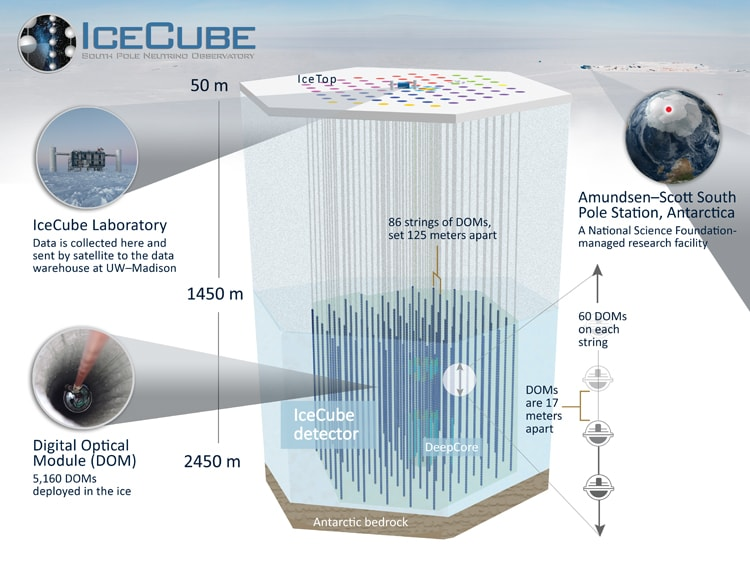
\includegraphics[width=12cm,keepaspectratio]{icecube_detector_schematic.jpeg}
  \caption{Schematic of the IceCube Experiment\cite{IceCube}.}
  \label{fig:IceCube}
\end{figure}

Consisting of the In-Ice Array~\cite{In-Ice}, IceTop~\cite{IceTop} and DeepCore~\cite{DeepCore}, the IceCube experiment is used to study neutrinos and muons. It is located at the Amundsen-Scott South Pole Station near the geographical south pople. The experiment consists of 5160 digital optical modules (DOMs) on 86 strings located $\SIrange{1450}{2450}{\metre}$ under the surface as seen in \autoref{fig:IceCube}. The DOMs are photomultipliers (PMTs) in a vacuumised sphere of glass. These are used to detect the Cherenkov radiation emitted by muons, electrons and tau leptons. Cherenkov radiation is emitted when a relativistic particle travels through a medium with a speed greater than the speed of light in the medium
\begin{equation*}
  c_n = \frac{c_0}{n},
\end{equation*}
where $c_0$ is the speed of light in the vaccum and $n$ is the refractive index of the medium.
The seven strings of DeepCore are as well as their PMTs are spaced more densely, resulting in a lower energy threshold of $\SI{10}{\giga\electronvolt}$ in contrast to a $\SI{100}{\giga\electronvolt}$ energy threshold of the rest of the In-Ice Arry. With the IceTop experiment located at the surface of the south pole air showers are studied. It also functions as a veto for the In-Ice Array.
Neutrinos are measured indirectly via the charged (CC) and neutral currents (NC)
\begin{align*}
&&  \nu_l(\bar{\nu}_l) + A \to l^{\pm} + X && \mathrm{(CC)}\\
&&  \nu_l(\bar{\nu}_l) + A \to \nu_l + X && \mathrm{(NC)}
\end{align*}
where $A$ is a particle the neutrino interacts with and $X$ is a resulting particle shower. Since electrons are highly ionising, they quickly deposit all their energy resulting in a sphere of Cherenkov radiation. The same can be observed for tau leptons because of their short lifetime. Therefore it cannot be distinguished between electron and tau neutrinos, except for the energy of a tau neutrino exceeding $\SI{1}{\peta\electronvolt}$ since then the cascade of the CC interaction and that of the tau lepton decay are spatially separated.
The signature of NC interactions of all lepton flavors induced by the hadron shower is also similar to that of electrons in the CC channel.
Cherenkov radiation emitted by muons is too weak to be detected, but a muon produces $e^+ e^-$ pairs along its way emitting detectable Cherenkov radiation. This results in a cone-like signature for muons.\\

For rejection of atmospheric muons, so called \textit{starting events} are used. Here the outer layers of the detector are used as a veto leading to a smaller effective detector volume, where all neutrino flavors contribute in the same way, meaning that a majority of events are NC processes and CC electron and tau neutrino interactions. These have good energy resolution, but lack a good angle resolution.

Muon tracks have a worse energy resolution, but a higher angle resolution and depending on their energy a higher range allowing to use the earth as shielding, because only muons from neutrino interactions can come from below the detector. To reject atmospheric muons, a cut on the zenith angle can be performed also leading to an enhanced detector volume since also muons from neutrino interactions outisde the detector can be considered. Assuming a perfect reconstruction algorithm, that cut would reject all atmospheric muons. While this is not the case, the cut on the zenith angle still enhances the signal to background ratio from $1 : 10^6$ to $1 : 10^3$. To further improve background rejection machine learning algorithms can be utilised, which is the aim of this analysis.
